\chapter{設計}
\label{chap:design}
本章ではRive日本語入力の全体の設計について述べる。

\newpage
\section{Rive日本語入力システム}
Rive日本語入力システムは以下のものによって構成されている
\begin{itemize}
  \item Rive Client
  \item Rive Server
  \item Rive Analytics
  \item Rive Batchprocessing
  \item Rive Webservice
\end{itemize}
これらのシステムがお互いに作用することで
Rive日本語入力システムを実現している。
\begin{figure}[htbp]
  \begin{center}
    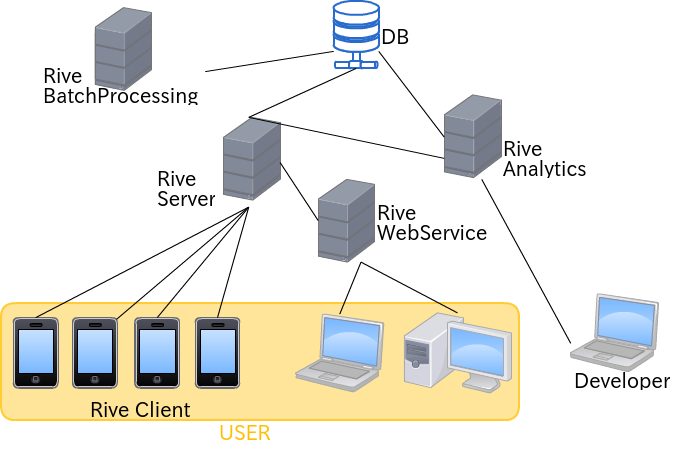
\includegraphics[width=12cm,bb=0 0 540 448]{images/systemstructure.png}
  \end{center}
  \caption{システム全体構成図}
  \label{fig:systemstructure}
\end{figure}

\section{Rive Client}
モバイルデバイスで利用可能なIMEアプリケーション本体。
ユーザーは基本的にこのアプリケーションのみを使用する。
システム全体の流れとしてRive Clientは
始めにRive Serverにコンテキストデータを送る。
またRive Serverから返ってきたデータを推薦候補単語としてユーザーに提示する。
(Rive Clientユーザ画面:\ref{fig:riveclient})
\begin{figure}
  \begin{center}
    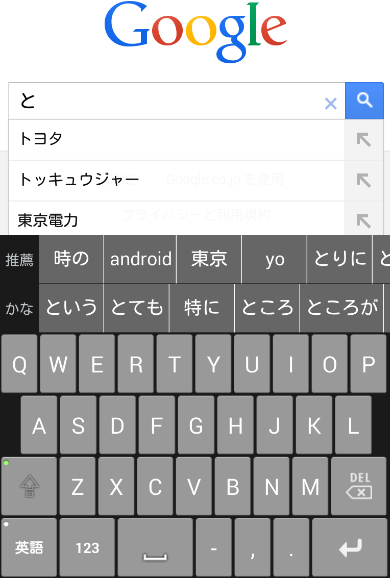
\includegraphics[width=140mm,bb=0 0 390 578]{images/riveclient.png}
  \end{center}
    \caption{Rive Clientユーザ画面}
    \label{fig:riveclient}
\end{figure}

\section{Rive Server}
Rive日本語入力における適切な候補単語を推測するサーバー郡の総称。
Rive Clientから受け取ったデータを解析し適切な推薦を行う。
また入力後のデータをRive Analyticsに送信するという役割も担っている。

\section{Rive Analytics}
文字入力のデータを受け取り解析することで開発者の手助けをするシステム。
バージョン管理システムであるgit\footnote{http://git-scm.com}
のcommit\footnote{http://git-scm.com/docs/git-commit}とデータを紐付けて
Rive日本語入力全体の有用性を確かめる為のシステム。
ユーザは本システムへの直接の関わりは持たない。

\section{Rive Batchprocessing}
定期的に処理を行うシステムの総称。
主にDBの更新、編集などを行うプログラムで構成されている。

\section{Rive Webservice}
システムを試用するためのWEBページとして実装。
仮想のコンテキストを設定し、どのような推薦候補単語を
受け取ることができるかシミュレーションすることができる。
またRive日本語入力の紹介も兼ねている。

\section{データベース}
取得するコンテキストと共に、
スキーマが頻繁に変わるため
スキーマの変更に対応しやすいNoSQLデータでーすである
MongoDBを採用した。

\section{システム間通信}
Rive ClientとRive Server間の通信は
Websocket\footnote{http://dev.w3.org/html5/websockets/}、
その他システム間はhttpによって実現した。
Websocketを採用した理由はサーバー側からのプッシュ機構を導入するためと、
httpより速度が早いためという理由である。\cite{websocket}
